\documentclass{beamer}
\let\vec\mathbf
\mode<presentation>
\usepackage{amsmath}
\usepackage{amssymb}
%\usepackage{advdate}
\usepackage{adjustbox}
%\usepackage{subcaption}
%\usepackage{enumitem}
\usepackage{multicol}
\usepackage{mathtools}
\usepackage{mathtools}
\DeclarePairedDelimiter{\abs}{\lvert}{\rvert}
\usepackage{listings}
\usepackage{url}
\usetheme{Boadilla}
\usecolortheme{lily}
\setbeamertemplate{footline}
{
  \leavevmode%
  \hbox{%
  \begin{beamercolorbox}[wd=\paperwidth,ht=2.25ex,dp=1ex,right]{author in head/foot}%
    \insertframenumber{} / \inserttotalframenumber\hspace*{2ex} 
  \end{beamercolorbox}}%
  \vskip0pt%
}
\setbeamertemplate{navigation symbols}{}
\providecommand{\nCr}[2]{\,^{#1}C_{#2}} % nCr
\providecommand{\nPr}[2]{\,^{#1}P_{#2}} % nPr
\providecommand{\mbf}{\mathbf}
\providecommand{\pr}[1]{\ensuremath{\Pr\left(#1\right)}}
\providecommand{\qfunc}[1]{\ensuremath{Q\left(#1\right)}}
\providecommand{\sbrak}[1]{\ensuremath{{}\left[#1\right]}}
\providecommand{\lsbrak}[1]{\ensuremath{{}\left[#1\right.}}
\providecommand{\rsbrak}[1]{\ensuremath{{}\left.#1\right]}}
\providecommand{\brak}[1]{\ensuremath{\left(#1\right)}}
\providecommand{\lbrak}[1]{\ensuremath{\left(#1\right.}}
\providecommand{\rbrak}[1]{\ensuremath{\left.#1\right)}}
\providecommand{\cbrak}[1]{\ensuremath{\left\{#1\right\}}}
\providecommand{\lcbrak}[1]{\ensuremath{\left\{#1\right.}}
\providecommand{\rcbrak}[1]{\ensuremath{\left.#1\right\}}}
\theoremstyle{remark}
\newtheorem{rem}{Remark}
\newcommand{\sgn}{\mathop{\mathrm{sgn}}}

\providecommand{\res}[1]{\Res\displaylimits_{#1}} 
\providecommand{\norm}[1]{\lVert#1\rVert}
\providecommand{\mtx}[1]{\mathbf{#1}}

\providecommand{\fourier}{\overset{\mathcal{F}}{ \rightleftharpoons}}
%\providecommand{\hilbert}{\overset{\mathcal{H}}{ \rightleftharpoons}}
\providecommand{\system}{\overset{\mathcal{H}}{ \longleftrightarrow}}
	%\newcommand{\solution}[2]{\textbf{Solution:}{#1}}
%\newcommand{\solution}{\noindent \textbf{Solution: }}
\providecommand{\dec}[2]{\ensuremath{\overset{#1}{\underset{#2}{\gtrless}}}}
\newcommand{\myvec}[1]{\ensuremath{\begin{pmatrix}#1\end{pmatrix}}}

\title{Matrices in Geometry - 8.4.38}
\author{EE25BTECH11035  Kushal B N}
\date{}

\begin{document}

\maketitle

\section{Problem Statement}
\begin{frame}
\frametitle{Problem Statement}
Let $0 < \theta < \frac{\pi}{2}$. If the eccentricity of the hyperbola $\frac{x^2}{\cos^2{\theta}} - \frac{y^2}{\sin^2{\theta}} = 1$ is greater than 2, then the length of its latus rectum lies in the interval
\begin{enumerate}
    \item $(5,\infty)$
    \item $(\frac{3}{2},3 ]$
    \item $(2,3]$
    \item $(1,\frac{3}{2}]$
\end{enumerate}
\end{frame}

\section{Solution}
\begin{frame}{Solution}
Given,
Hyperbola $\sec^2(\theta)x^2 - \csc^2(\theta)y^2 = 1$ for which $e>2$.

Comparing to the general conic form $\vec{x}^{\top}\vec{V}\vec{x} + 2\vec{u}^{\top}\vec{x} + f = 0$, we get

\begin{equation}
    \vec{V} = \myvec{\sec^2(\theta) & 0\\0 & \csc^2(\theta)}
\end{equation}

\begin{equation}
    \vec{u} = \myvec{0\\0}
\end{equation}

\begin{equation}
    f = -1
\end{equation}

Now, here as $\vec{V}$ is a diagonal matrix, its eigenvalues are its diagonal entries, that is,
\begin{equation}
    \lambda_1 = \frac{1}{\sin^2{\theta}}
\end{equation}
\begin{equation}
    \lambda_2 = \frac{1}{\cos^2{\theta}}
\end{equation}
\end{frame}

\begin{frame}{Solution}
Now, the eccentricity of the hyperbola
\begin{equation}
    e = \sqrt{1 - \frac{\lambda_1}{\lambda_2}}
\end{equation}

\begin{equation}
    \implies e^2 = 1 + \frac{\sin^2{\theta}}{\cos^2{\theta}} = \frac{1}{\cos^2{\theta}}
\end{equation}

As $0 < \theta < \frac{\pi}{2}$, $\cos{\theta}$ is positive and so,
\begin{equation}
    e = \frac{1}{\cos{\theta}}
\end{equation}

Now, as $e > 2$
\begin{equation}
    \frac{1}{\cos{\theta}} > 2 \implies \cos{\theta} < \frac{1}{2}
\end{equation}

\begin{equation}
    \implies \frac{\pi}{3} < \theta < \frac{\pi}{2}
    \label{eq10}
\end{equation}
\end{frame}

\begin{frame}{Solution}
Length of the latus rectum,
\begin{equation}
    l = \frac{2\sqrt{\abs{f_0\lambda_1}}}{\abs{\lambda_2}}
    \label{eq11}
\end{equation}

where,
\begin{equation}
    f_0 = \vec{u}^{\top}\vec{V}^{-1}\vec{u} - f
\end{equation}

as $\vec{u} = \myvec{0\\0}$, we get
\begin{equation}
    f_0 = -f = -(-1) = 1
\end{equation}

Substituting these values into \eqref{eq11}, we get
\begin{equation}
    l = \frac{2\sqrt{\abs{1.\sec^2\theta}}}{\abs{\csc^2\theta}}
\end{equation}
\end{frame}

\begin{frame}{Solution}
    In the interval $0 < \theta < \frac{\pi}{2}$, $\sec\theta$ is positive and so
\begin{equation}
    \implies l = \frac{2\sin^2{\theta}}{\cos{\theta}}
\end{equation}

Now from \eqref{eq10}, we get
\begin{equation}
    \fbox{$l \in (3,\infty)$}
\end{equation}
\end{frame}

\section{Conclusion}
\begin{frame}{Conclusion}
$\therefore$ The length of the latus rectum for the given hyperbola lies in the interval $(3,\infty)$.

\begin{figure}[H]
    \centering
    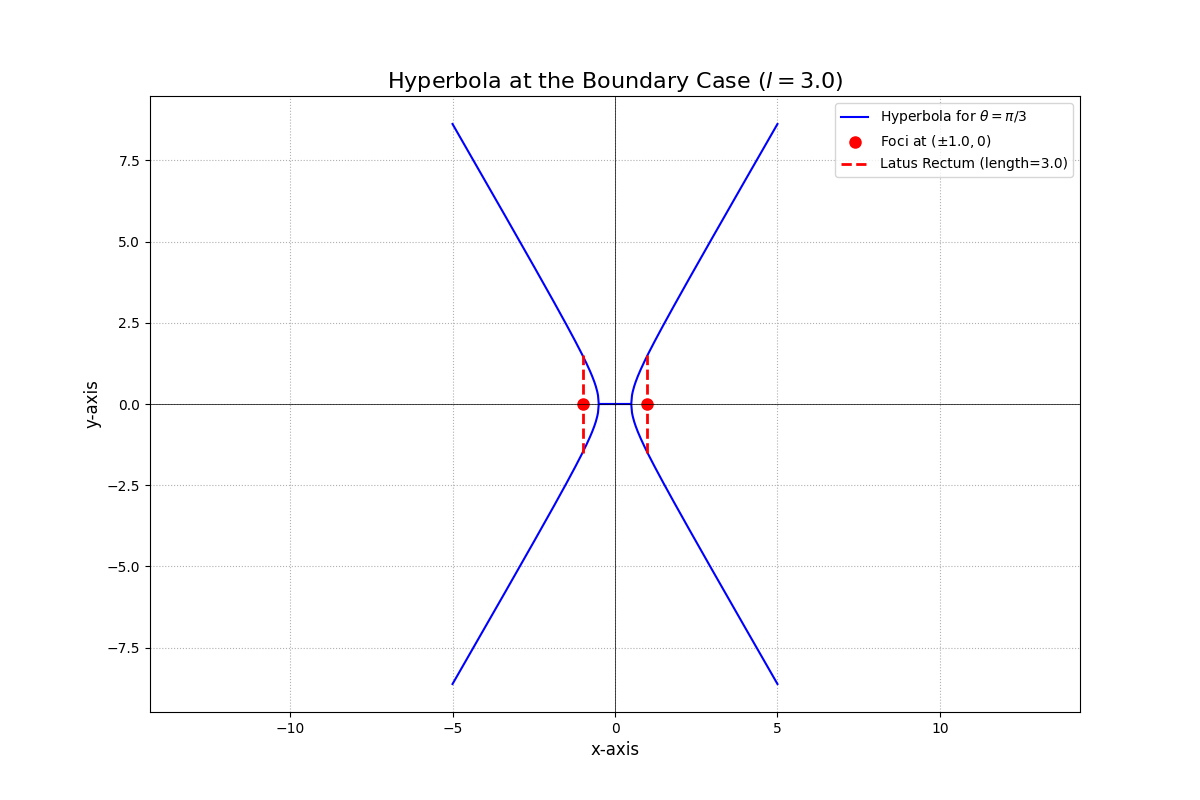
\includegraphics[width=0.60\columnwidth]{figs/1.png}
    \caption{Plot for 8.4.38}
\end{figure}
\end{frame}
\end{document}
